\documentclass[twoside, 11pt]{article}
% ========== Packages ==========
\usepackage[a4paper,
  left=25mm,
  right=25mm,
  top=30mm,
  bottom=35mm,
  headheight=35mm
]{geometry}

\usepackage[ngerman]{babel} %Ändert die Sprache
\usepackage[T1]{fontenc} %Wichtig für ä ö ü
\usepackage{amssymb} %Für mathematische Zeichen
\usepackage{amsthm} %Für mathematische Umgebungen
\usepackage{graphicx}
\usepackage{fancyhdr}
\usepackage[utf8]{inputenc}
\usepackage{multirow} %Für Tabellen
\usepackage{longtable} %Für lange Tabellen
\usepackage{tabularx}
\usepackage{pdfpages} %Zum einfügen von PDF's
\usepackage{hyperref} %Für hyperlinks
\hypersetup{bookmarks=true}
\usepackage{parskip}
\usepackage{caption} %Für die Beschriftung von Bilder
\captionsetup{justification=centering}
\captionsetup{font=it}
\setlength{\parindent}{0pt}
\usepackage{subcaption} %Für die Beschriftung unterteilter Bilder
\usepackage{float}
\floatstyle{plaintop}
\restylefloat{table}

\makeatletter %Für römische Zahlen
\newcommand*{\rom}[1]{\expandafter\@slowromancap\romannumeral #1@}

%Für die dicken Linien in Tabellen
\def\thickhline{%
  \noalign{\ifnum0=`}\fi\hrule \@height \thickarrayrulewidth \futurelet
   \reserved@a\@xthickhline}
\def\@xthickhline{\ifx\reserved@a\thickhline
               \vskip\doublerulesep
               \vskip-\thickarrayrulewidth
               \fi
      \ifnum0=`{\fi}}
\makeatother
\newlength{\thickarrayrulewidth}
\setlength{\thickarrayrulewidth}{2\arrayrulewidth}

%Sorgt dafür, dass nicht immer alles auf die ganze Seite verteilt wird.
\raggedbottom

% ========== Header and Footer ==========
\pagestyle{fancy}
\fancyhf{}
\fancyhead[RE,LO]{Seite \thepage}
\fancyhead[LE,RO]{\nouppercase{\leftmark}}
\fancyfoot[RE,LO]{BAT FS21}

%Eigens erstellte Variablen
\newcommand{\plotWidth}{0.7}
\newcommand{\garphWidth}{0.7}


\begin{document}
% ==================== Titelseite ====================
  \begin{titlepage}
    \begin{center}
        % \vspace*{1cm}

        \LARGE
        Bachelor-Thesis an der Hochschule Luzern\\
        Technik \& Architektur

        \vspace{0.8cm}
        \Huge
        \textbf{Solar Butterfly - Auslegung Grundstruktur}

        \vspace{3cm}

        \begin{center}
          \makebox[\textwidth]{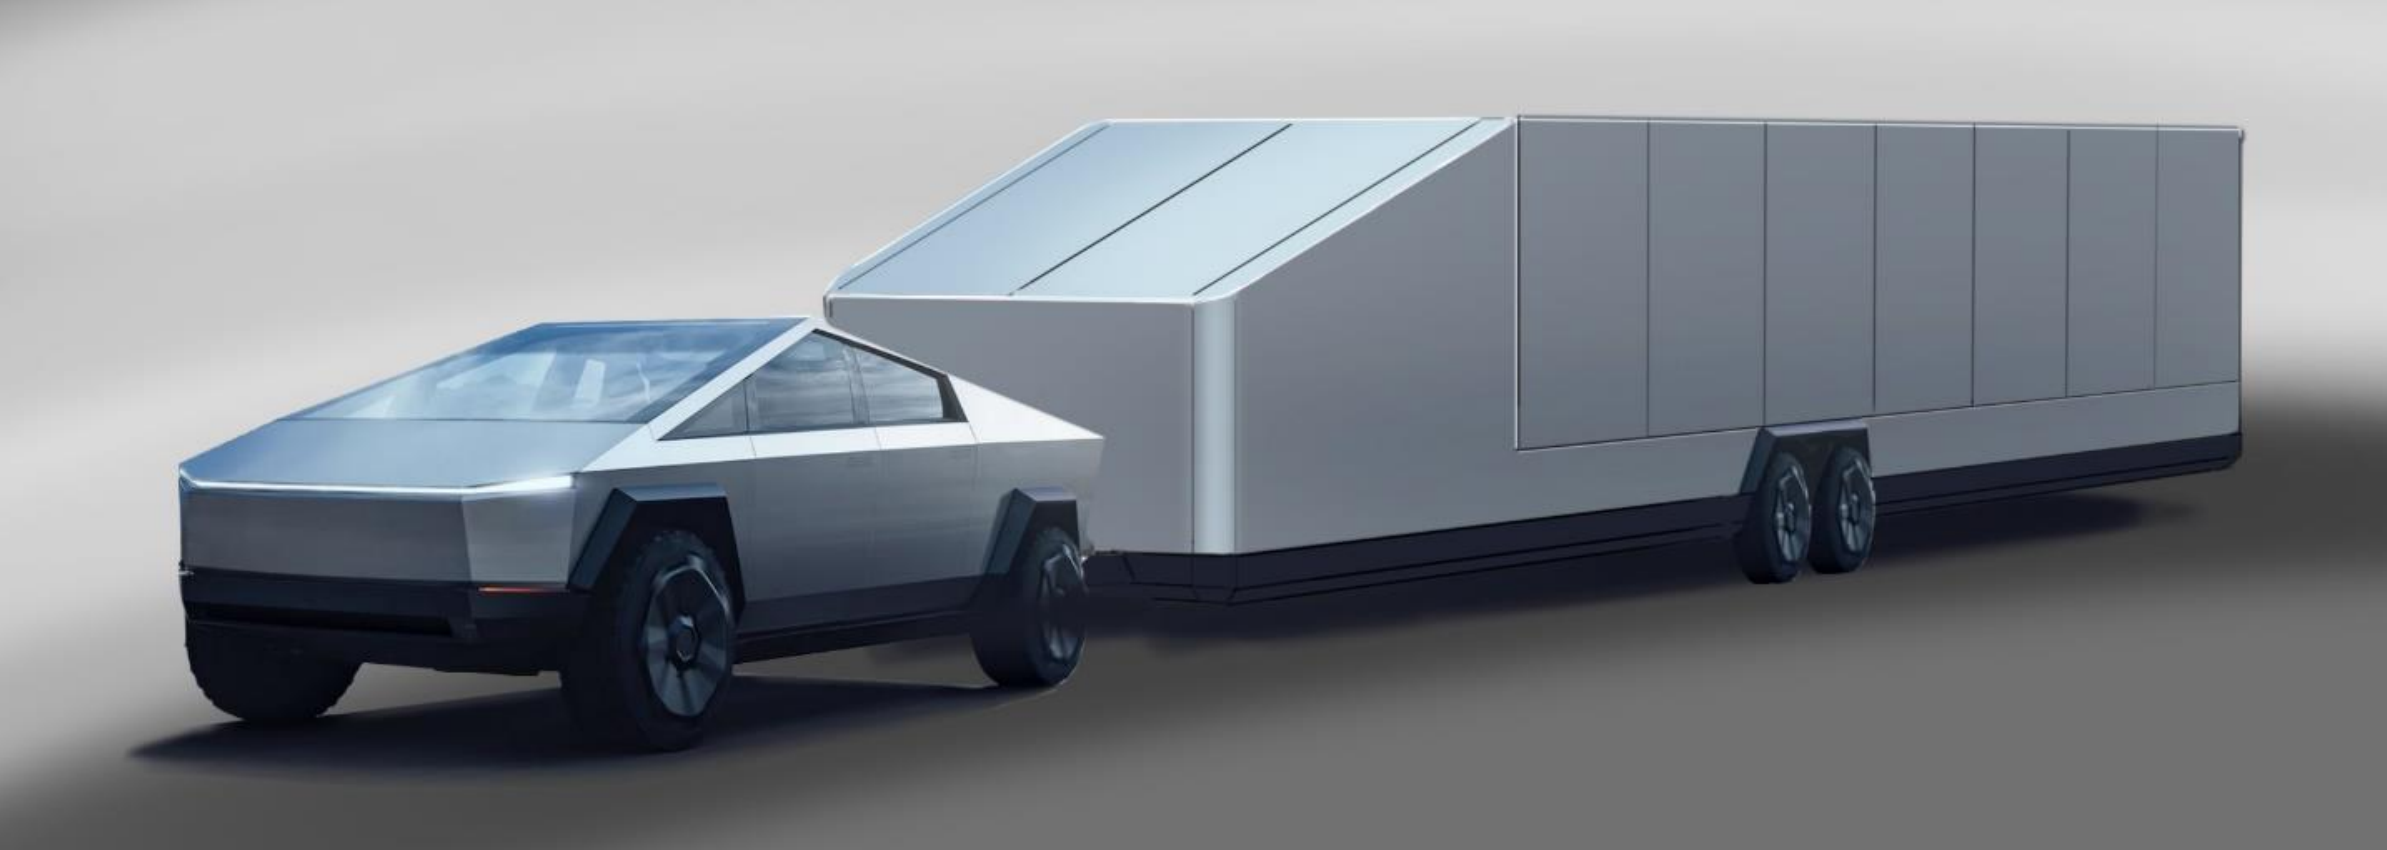
\includegraphics[width=1\paperwidth]{04_Figures/SB0.png}}
        \end{center}

        \vfill
        \begin{table}[b]
        \small
          \begin{tabularx}{\linewidth}{llX}
            \textbf{Diplomandin/Diplomand} & \textbf{Gut, Andre}                                &\\[4 mm]
            \textbf{Bachelor-Studiengang}  & \textbf{Bachelor Maschinentechnik}                 &\\[4 mm]
            \textbf{Semester}              & \textbf{FS21}                                      &\\[4 mm]
            \textbf{Dozentin/Dozent}       & \textbf{Roman\v{c}uk, Dejan}                       &\\[4 mm]
            \textbf{Expertin/Experte}      & \textbf{Dubach, Roger}                             &
          \end{tabularx}
        \end{table}

    \end{center}
\end{titlepage}


% ==================== Frontmatter ====================
  \pagenumbering{roman}
  \setcounter{page}{2}

  \vspace{2cm}
\begin{large}
\textbf{Bachelor-Thesis an der Hochschule Luzern - Technik \& Architektur}\\
\end{large}
\vspace{1cm}

\begin{table}[H]
\small
  \begin{tabularx}{\linewidth}{llX}
    \textbf{Titel}                 & \textbf{Solar Butterfly - Auslegung Grundstruktur} &\\[4 mm]
    \textbf{Diplomandin/Diplomand} & \textbf{Gut, Andre}                                &\\[4 mm]
    \textbf{Bachelor-Studiengang}  & \textbf{Bachelor Maschinentechnik}                 &\\[4 mm]
    \textbf{Semester}              & \textbf{FS21}                                      &\\[4 mm]
    \textbf{Dozentin/Dozent}       & \textbf{Roman\v{c}uk, Dejan}                       &\\[4 mm]
    \textbf{Expertin/Experte}      & \textbf{Dubach, Roger}                             &
  \end{tabularx}
\end{table}

\vspace{1.5cm}
\textbf{Abstract Deutsch}\\
Ziel des Projektes \emph{Solar Butterfly} ist die Entwicklung eines autarken Wohnwagens, welcher sich mit selbst erzeugten Solarstrom versorgen und autonom operiert werden kann. Der Solar Butterfly soll international Aufmerksamkeit erregen und so nachhaltige Lösungen im Bereich des Klimaschutzes und Elektromobilität ermutigen und vorantreiben. In Zusammenarbeit mit drei weiteren Maschinenbaustudenten und deren Bachelorarbeiten soll die Vision des Solar Butterflys in die Realität umgesetzt werden.\\
Diese Arbeit befasst sich mit dem Definieren der Anforderungen und Auslegungskriterien des Solar Butterflys, dem Bestimmen von Design-Allowables, der Ausarbeitung eines Lastenheftes und der Grobauslegung der Grundstruktur. Zur Bestimmung von Schnittgrössen soll dabei ein globales FEM-Modell zur Anwendung kommen.\\
Handrechnungen und FEM-Berechnungen zeigen, dass von den untersuchten Belastungen die Lastfälle der vertikalen und rotatorischen Beschleunigung, welche während der Fahrt auftreten, die grössten Beanspruchungen darstellen. Zugleich weisen diese Lastfälle aufgrund von nur bedingt abschätzbaren Randbedingungen die grössten Unsicherheiten und Risiken auf. Weiter konnte in Erfahrung gebracht werden, dass die Klebeverbindung zwischen dem Boden und Chassis als Kritisch zu beurteilen ist und dass weitere Untersuchungen und Abklärungen diesbezüglich nötig sind.
Ferner konnte Potential zur Gewichtsreduktion in Form einer Optimierung des Chassis in Verbindung mit dem Boden ausfindig gemacht werden.


\textbf{Abstract Englisch}\\
The goal of the project \emph{Solar Butterfly} is the development of a self-sufficient caravan, which can be powered by self-generated solar electricity and operate autonomously. The Solar Butterfly is intended to attract international attention and thus encourage and promote sustainable solutions in the field of climate protection and electromobility. In collaboration with three
other mechanical engineering students and their bachelor thesis, the vision of the Solar Butterfly is to be turned into reality.
This work deals with the definition of the requirements and design criteria for the Solar Butterfly, the specification of design allowables, the elaboration of a specification sheet and the rough design of the basic structure. A global FEM model will be used to determine the sectional forces.
Hand calculations and FEM calculations show that of the loads investigated, the load cases of vertical and rotational acceleration, which occur during driving, represent the greatest stresses. It was also found that the adhesive bond between the floor and the chassis is critical and that further investigations and clarifications are necessary. Furthermore, potential for weight reduction could be identified by optimizing the chassis in conjunction with the floor.

\vspace{2cm}
Ort, Datum $\;\;\;\;\;\;\;\;\;\;\;\;\;\;\;\;\;\;\;\;$ Luzern, 11. Juni 2021\\
\textbf{{\small $^\copyright$} Andre Gut, Hochschule Luzern - Technik \& Architektur}

\vspace*{\fill}

\noindent
{\color{gray} \rule{\linewidth}{0.5px} }
\begin{footnotesize}
  \textcolor{gray}{Alle Rechte vorbehalten. Die Arbeit oder Teile davon dürfen ohne schriftliche Genehmigung der Rechteinhaber weder in irgendeiner Form reproduziert noch elektronisch gespeichert, verarbeitet, vervielfältigt oder verbreitet werden.}\\
  \textcolor{gray}{Sofern die Arbeit auf der Website der Hochschule Luzern online veröffentlicht wird, können abweichende Nutzungsbedingungen unter Creative-Commons-Lizenzen gelten. Massgebend ist in diesem Fall die auf der Website angezeigte Creative-Commons-Lizenz.}
\end{footnotesize}
\newpage

  \textbf{Abstract Deutsch}\\
Ziel des Projektes \emph{Solar Butterfly} ist die Entwicklung eines autarken Wohnwagens, welcher sich mit selbst erzeugten Solarstrom versorgen und autonom operiert werden kann. Der Solar Butterfly soll international Aufmerksamkeit erregen und so nachhaltige Lösungen im Bereich des Klimaschutzes und Elektromobilität ermutigen und vorantreiben. In Zusammenarbeit mit drei weiteren Maschinentechnikstudenten und deren Bachelor-Thesen soll die Vision des Solar Butterflys in die Realität umgesetzt werden.\\
Diese Arbeit befasst sich mit dem Definieren der Anforderungen und Auslegungskriterien des Solar Butterflys, dem Bestimmen von Design-Allowables, der Ausarbeitung eines Lastenheftes und der Grobauslegung der Grundstruktur. Zur Bestimmung von Schnittgrössen soll dabei ein globales FEM-Modell zur Anwendung kommen.\\
Handrechnungen und FEM-Berechnungen zeigen, dass von den untersuchten Belastungen die Lastfälle der vertikalen und rotatorischen Beschleunigung, welche während der Fahrt auftreten, die grössten Beanspruchungen darstellen. Zugleich weisen diese Lastfälle aufgrund von nur bedingt abschätzbaren Randbedingungen die grössten Unsicherheiten und Risiken auf. Weiter konnte in Erfahrung gebracht werden, dass die Klebeverbindung zwischen dem Boden und Chassis als Kritisch zu beurteilen ist und dass weitere Untersuchungen und Abklärungen diesbezüglich nötig sind.
Ferner konnte Potential zur Gewichtsreduktion in Form einer Optimierung des Chassis in Verbindung mit dem Boden ausfindig gemacht werden.


\textbf{Abstract Englisch}\\
The goal of the project \emph{Solar Butterfly} is the development of a self-sufficient caravan, which can supply itself with self-generated solar power and be operated autonomously. The Solar Butterfly is intended to draw international attention and thus encourage and promote sustainable solutions in the field of climate protection and electromobility. In collaboration with three other mechanical engineering students and their bachelor thesis, the vision of the Solar Butterfly is to be turned into reality.\\
This thesis deals with the definition of the requirements and design criteria of the Solar Butterfly, the determination of design allowables, the elaboration of a specification sheet and the rough dimensioning of the basic structure. A global FEM model is to be used to determine cutting forces.\\
Manual calculations and FEM simulations show that of the loads investigated, the load cases of vertical and rotational acceleration, which occur while the vehicle is moving, represent the greatest stresses. At the same time, these load cases show the greatest uncertainties and risks due to boundary conditions which can only be estimated to a limited extent. It was also found that the adhesive bond between the floor and the chassis is critical and that further investigations and clarifications are necessary in this respect.\\
Furthermore, potential for weight reduction in the form of an optimization of the chassis in conjunction with the floor was identified.

\vspace{2cm}
Ort, Datum $\;\;\;\;\;\;\;\;\;\;\;\;\;\;\;\;\;\;\;\;$ Luzern, 11. Juni 2021\\
\textbf{{\small $^\copyright$} Andre Gut, Hochschule Luzern - Technik \& Architektur}

\vspace*{\fill}

\noindent
{\color{gray} \rule{\linewidth}{0.5px} }
\begin{footnotesize}
  \textcolor{gray}{Alle Rechte vorbehalten. Die Arbeit oder Teile davon dürfen ohne schriftliche Genehmigung der Rechteinhaber weder in irgendeiner Form reproduziert noch elektronisch gespeichert, verarbeitet, vervielfältigt oder verbreitet werden.}\\
  \textcolor{gray}{Sofern die Arbeit auf der Website der Hochschule Luzern online veröffentlicht wird, können abweichende Nutzungsbedingungen unter Creative-Commons-Lizenzen gelten. Massgebend ist in diesem Fall die auf der Website angezeigte Creative-Commons-Lizenz.}
\end{footnotesize}
\newpage


% ==================== Table of contents ====================
  \tableofcontents
  \newpage

% ==================== Mainmatter ====================
  \pagenumbering{arabic}
  \setcounter{page}{1}
  \part{Dokumentation}


% ==================== Backmatter ====================
  \part{Anhang}
  \appendix
  \section{Quellenverzeichnis}

\renewcommand\refname{\vskip -1cm}
\bibliography{03_Backmatter/mybib}
\bibliographystyle{ieeetr}

  \section{Abbildungsverzeichnis}
\renewcommand\listfigurename{}
\vspace*{-1cm}
\listoffigures

  \section{Tabellenverzeichnis}
\renewcommand\listtablename{}
\vspace*{-1cm}
\listoftables
\newpage

  \section{Lastenheft}
  \subsection{Berechnung der Vertikalen Beschleunigung}
  Die Position des Rades während dem Überfahren der Bremsschwelle ist gegeben durch folgenden Zusammenhang:
  \begin{equation}
    x_r^n = h \cdot sin\left(\pi \cdot \frac{n \cdot \Delta t \cdot v}{l}\right)
  \end{equation}
  $l$ steht dabei für die Länge, und h für die Höhe der Bremsschwelle. $v$ für die Geschwindigkeit des Solar Butterflys beim Überfahren, $n$ für den Zeitschritt und $\Delta t$ für die Zeitinkrementierung pro Berechnungsschritt.\\

  Um die Beschleunigung des Solar Butterflys zu berechnen, wird in einem ersten Schritt dessen Position zum Zeitpunk $n$ $x_{SB}^n$ aus der vorangehenden Situation berechnet.
  \begin{equation}
    x_{SB}^n = x_{SB}^{(n-1)} + v^{(n-1)} \cdot \Delta t
  \end{equation}

  Als nächstes wird der Federweg $s^n$, sowie die Änderungsrate des Federwegs $v_s^n$ zum Zeitpunkt $n$ aus den Positionen des Rades $r_x^n$ und des Solar Butterflys $x_{SB}^n$ berechnet.
  \begin{equation}
    s^n = x_r^n - x_{SB}^n
  \end{equation}
  \begin{equation}
    v_s^n = \frac{s^n - s^{(n-1)}}{\Delta t}
  \end{equation}

  Die Beschleunigung des Solar Butterfly ergibt sich dann zu:\\
  \begin{equation}
    a_{SB}^n = \frac{k \cdot s^n + d \cdot v_s^n}{m}
  \end{equation}

  Wobei $k$ für die Federkonstante und $d$ für die Dämpfungskonstante stehen.
  Die aus der Beschleunigung des Solar Butterfly resultierende neue Geschwindigkeit, kann wie folgt berechnet werden.
  \begin{equation}
    v^n = v^{(n-1)} + a_{SB}^n \cdot \Delta t
  \end{equation}



\section{FEM}

\subsection{FEM Ergebnisse}
  \label{FEM Ergebnisse}

  \subsubsection{FEM-Ergebnis - Lastfall 1.1 Vertikale Beschleunigung}
  \begin{table}[H]
  \centering
  \begin{tabular}{lcccccc}
  Grösse	&	Einheit	&	x	&	y	&	z	&	Total	&	Berechnet	\\	\hline
  \multicolumn{5}{l}{\textbf{Lagerreaktionen}}									&		&		\\	\thickhline
  Deichsel	&	N	&	0	&	3193	&	0	&	3193	&	-1028	(y) \\
  Chassis Links	&	N	&	0	&	35171	&	6733	&	35810	&	37300 (y)	\\
  Chassis Rechts	&	N	&	0	&	35171	&	-6733	&	35810	&	37300 (y)	\\	\hline	\\
  \multicolumn{5}{l}{\textbf{Chassis}}									&		&		\\	\thickhline
  Axialkraft	&	N	&		&		&		&	-50730	&	-44518	\\
  Querkraft	&	N	&		&		&		&	17003	&	19079	\footnotemark \\
  Biegemoment	&	kNmm	&		&		&		&	16980	&		\\	\hline	\\
  \multicolumn{5}{l}{\textbf{Dach}}									&		&		\\	\thickhline
  Axialkraft	&	N	&		&		&		&	2879	&	14840	\\
  Querkraft	&	N	&		&		&		&	108	&		\\
  Biegemoment	&	kNmm	&		&		&		&	42	&		\\	\hline	\\
  \multicolumn{5}{l}{\textbf{Träger A und B}}													\\	\thickhline
  Axialkraft	&	N	&		&		&		&	-10904	&		\\
  Querkraft	&	N	&		&		&		&	1293	&		\\
  Biegemoment	&	kNmm	&		&		&		&	327	&		\\	\hline	\\
  \multicolumn{5}{l}{\textbf{Kontaktreaktion: Chassis - Träger A und B}}									&		&		\\	\thickhline
   Axialkraft A	&	N	&	-620	&	12931	&	-218	&	12948	&		\\
  Biegemoment A	&	kNmm	&	-4602	&	-179	&	341	&	4618	&		\\
  Axialkraft B	&	N	&	2464	&	15784	&	713	&	15991	&		\\
  Biegemoment B	&	kNmm	&	-5610	&	851	&	-346	&	5685	&		\\	\hline	\\
  \multicolumn{5}{l}{\textbf{Kontaktreaktion: Chassis - Boden}}									&		&		\\	\thickhline
  Normalkraft (Zug)	&	N	&		&		&		&	883	&		\\
  Schubkraft (xz-Ebene)	&	N	&		&		&		&	9933	&		\\	\hline
  \end{tabular}
  \caption{Resultate der FEM-Simulation des Lastafalles der vertikalen Beschleunigung}
  \label{tab:FEM 1.1}
  \end{table}
  \footnotetext[2]{Unter der Annahme, dass nur das Chassis Querkräfte aufnimmt. Die Kraft von 19 kN ergibt sich aus der Halbierung der globalen Querkraft aus der Berechnung im Kapitel \ref{1.1 Vertikale Beschleunigung}.}

  \subsubsection{FEM-Ergebnis - Lastfall 1.3 Longitudinale Beschleunigung negativ}
  \begin{table}[H]
  \centering
  \begin{tabular}{lcccccc}
  Grösse	&	Einheit	&	x	&	y	&	z	&	Total	&	Berechnet	\\	\hline
  \multicolumn{5}{l}{\textbf{Lagerreaktionen}}									&		&		\\	\thickhline
  Deichsel	&	N	&	-20611	&	-3050	&	0	&	20835	&	206000 (x)	\\
  Chassis Links	&	N	&	0	&	1525	&	515	&	1610	&		\\
  Chassis Rechts	&	N	&	0	&	1525	&	-515	&	1610	&		\\	\hline	\\
  \multicolumn{5}{l}{\textbf{Chassis}}									&		&		\\	\thickhline
  Axialkraft	&	N	&		&		&		&	6080	&		\\
  Querkraft	&	N	&		&		&		&	1319	&		\\
  Biegemoment	&	kNmm	&		&		&		&	2601	&		\\	\hline	\\
  \multicolumn{5}{l}{\textbf{Dach}}									&		&		\\	\thickhline
  Axialkraft	&	N	&		&		&		&	553	&		\\
  Querkraft	&	N	&		&		&		&	8	&		\\
  Biegemoment	&	kNmm	&		&		&		&	2	&		\\	\hline	\\
  \multicolumn{5}{l}{\textbf{Träger A und B}}													\\	\thickhline
  Axialkraft	&	N	&		&		&		&	-1562	&		\\
  Querkraft	&	N	&		&		&		&	56	&		\\
  Biegemoment	&	kNmm	&		&		&		&	17	&		\\	\hline	\\
  \multicolumn{5}{l}{\textbf{Kontaktreaktion: Chassis - Träger A und B}}									&		&		\\	\thickhline
   Axialkraft A	&	N	&	-56	&	2084	&	325	&	2110	&		\\
  Biegemoment A	&	kNmm	&	-734	&	-19	&	2	&	734	&		\\
  Axialkraft B	&	N	&	98	&	667	&	80	&	679	&		\\
  Biegemoment B	&	kNmm	&	-236	&	34	&	-14	&	238	&		\\	\hline	\\
  \multicolumn{5}{l}{\textbf{Kontaktreaktion: Chassis - Boden}}									&		&		\\	\thickhline
  Normalkraft (Zug)	&	N	&		&		&		&	35	&		\\
  Schubkraft (xz-Ebene)	&	N	&		&		&		&	1733	&		\\	\hline
  \end{tabular}
  \caption{Resultate der FEM-Simulation des Lastafalles der longitudinalen Beschleunigung}
  \label{tab:FEM 1.3}
  \end{table}


  \subsubsection{FEM-Ergebnis - Lastfall 1.4 laterale Beschleunigung}
  \begin{table}[H]
  \centering
  \begin{tabular}{lcccccc}
  Grösse	&	Einheit	&	x	&	y	&	z	&	Total	&	Berechnet	\\	\hline
  \multicolumn{5}{l}{\textbf{Lagerreaktionen}}									&		&		\\	\thickhline
  Deichsel	&	N	&	0	&	0	&	1023	&	1023	&	-330 (z)	\\
  Chassis Links	&	N	&	0	&	-15008	&	11290	&	18780	&	11900 (z)	\\
  Chassis Rechts	&	N	&	0	&	15008	&	11242	&	18752	&	11900 (z)	\\	\hline	\\
  \multicolumn{5}{l}{\textbf{Chassis}}									&		&		\\	\thickhline
  Axialkraft	&	N	&		&		&		&	-31674	&	-11480	\\
  Querkraft	&	N	&		&		&		&	7163	&	6100	\footnotemark \\
  Biegemoment	&	kNmm	&		&		&		&	6658	&		\\	\hline	\\
  \multicolumn{5}{l}{\textbf{Dach}}									&		&		\\	\thickhline
  Axialkraft	&	N	&		&		&		&	-2560	&	-964	\\
  Querkraft	&	N	&		&		&		&	24	&		\\
  Biegemoment	&	kNmm	&		&		&		&	13	&		\\	\hline	\\
  \multicolumn{5}{l}{\textbf{Träger A und B}}													\\	\thickhline
  Axialkraft	&	N	&		&		&		&	2684	&		\\
  Querkraft	&	N	&		&		&		&	1067	&	470	\\
  Biegemoment	&	kNmm	&		&		&		&	627	&	470	\\	\hline	\\
  \multicolumn{5}{l}{\textbf{Kontaktreaktion: Chassis - Träger A und B}}									&		&		\\	\thickhline
   Axialkraft A	&	N	&	237	&	-3577	&	1729	&	3979	&		\\
  Biegemoment A	&	kNmm	&	1924	&	71	&	-102	&	1928	&		\\
  Axialkraft B	&	N	&	-733	&	-4221	&	1679	&	4602	&		\\
  Biegemoment B	&	kNmm	&	2097	&	-251	&	95	&	2114	&		\\	\hline	\\
  \multicolumn{5}{l}{\textbf{Kontaktreaktion: Chassis - Boden}}									&		&		\\	\thickhline
  Normalkraft (Zug)	&	N	&		&		&		&	1942	&		\\
  Schubkraft (xz-Ebene)	&	N	&		&		&		&	10972	&		\\	\hline
  \end{tabular}
  \caption{Resultate der FEM-Simulation des Lastafalles der lateralen Beschleunigung}
  \label{tab:FEM 1.4}
  \end{table}
  \footnotetext[3]{Unter der Annahme, dass nur das Chassis Querkräfte aufnimmt. Die Kraft von 6.1 kN ergibt sich aus der Halbierung der globalen Querkraft aus der Berechnung im Kapitel \ref{1.4 Laterale Beschleunigung}.}


  \subsubsection{FEM-Ergebnis - Lastfall 1.5 Rotatorische Beschleunigung}
  \begin{table}[H]
  \centering
  \begin{tabular}{lcccccc}
  Grösse	&	Einheit	&	x	&	y	&	z	&	Total	&	Berechnet	\\	\hline
  \multicolumn{5}{l}{\textbf{Lagerreaktionen}}									&		&		\\	\thickhline
  Deichsel	&	N	&	0	&	0	&	804	&	804	&		\\
  Chassis Links	&	N	&	0	&	-23097	&	10913	&	25546	&	-27000 (y)	\footnotemark \\
  Chassis Rechts	&	N	&	0	&	23097	&	10844	&	25516	&	27000 (y)	\\	\hline	\\
  \multicolumn{5}{l}{\textbf{Chassis}}									&		&		\\	\thickhline
  Axialkraft	&	N	&		&		&		&	-44164	&		\\
  Querkraft	&	N	&		&		&		&	10927	&		\\
  Biegemoment	&	kNmm	&		&		&		&	10218	&		\\	\hline	\\
  \multicolumn{5}{l}{\textbf{Dach}}									&		&		\\	\thickhline
  Axialkraft	&	N	&		&		&		&	-3625	&		\\
  Querkraft	&	N	&		&		&		&	32	&		\\
  Biegemoment	&	kNmm	&		&		&		&	19	&		\\	\hline	\\
  \multicolumn{5}{l}{\textbf{Träger A und B}}													\\	\thickhline
  Axialkraft	&	N	&		&		&		&	-4119	&		\\
  Querkraft	&	N	&		&		&		&	1311	&		\\
  Biegemoment	&	kNmm	&		&		&		&	772	&		\\	\hline	\\
  \multicolumn{5}{l}{\textbf{Kontaktreaktion: Chassis - Träger A und B}}									&		&		\\	\thickhline
   Axialkraft A	&	N	&	373	&	-5525	&	2346	&	6014	&		\\
  Biegemoment A	&	kNmm	&	2767	&	112	&	-164	&	2774	&		\\
  Axialkraft B	&	N	&	-1309	&	-6399	&	2221	&	6899	&		\\
  Biegemoment B	&	kNmm	&	2996	&	-452	&	159	&	3034	&		\\	\hline	\\
  \multicolumn{5}{l}{\textbf{Kontaktreaktion: Chassis - Boden}}									&		&		\\	\thickhline
  Normalkraft (Zug)	&	N	&		&		&		&	3118	&		\\
  Schubkraft (xz-Ebene)	&	N	&		&		&		&	10761	&		\\	\hline
  \end{tabular}
  \caption{Resultate der FEM-Simulation des Lastafalles der rotatorischen Beschleunigung}
  \label{tab:FEM 1.5}
  \end{table}
  \footnotetext[4]{Die Kräfte von  $\pm$ 27 kN ergeben sich aus der Halbierung der Kraft F aus der Berechnung im Kapitel \ref{1.5 Rotatorische Beschleunigung}.}
    \newpage

\subsection{Deformationen}
\label{FEM Deformation}
\subsubsection{Deformation - Lastfall 1.1 Vertikale Beschleunigung}
\begin{figure}[H]
  \centering
  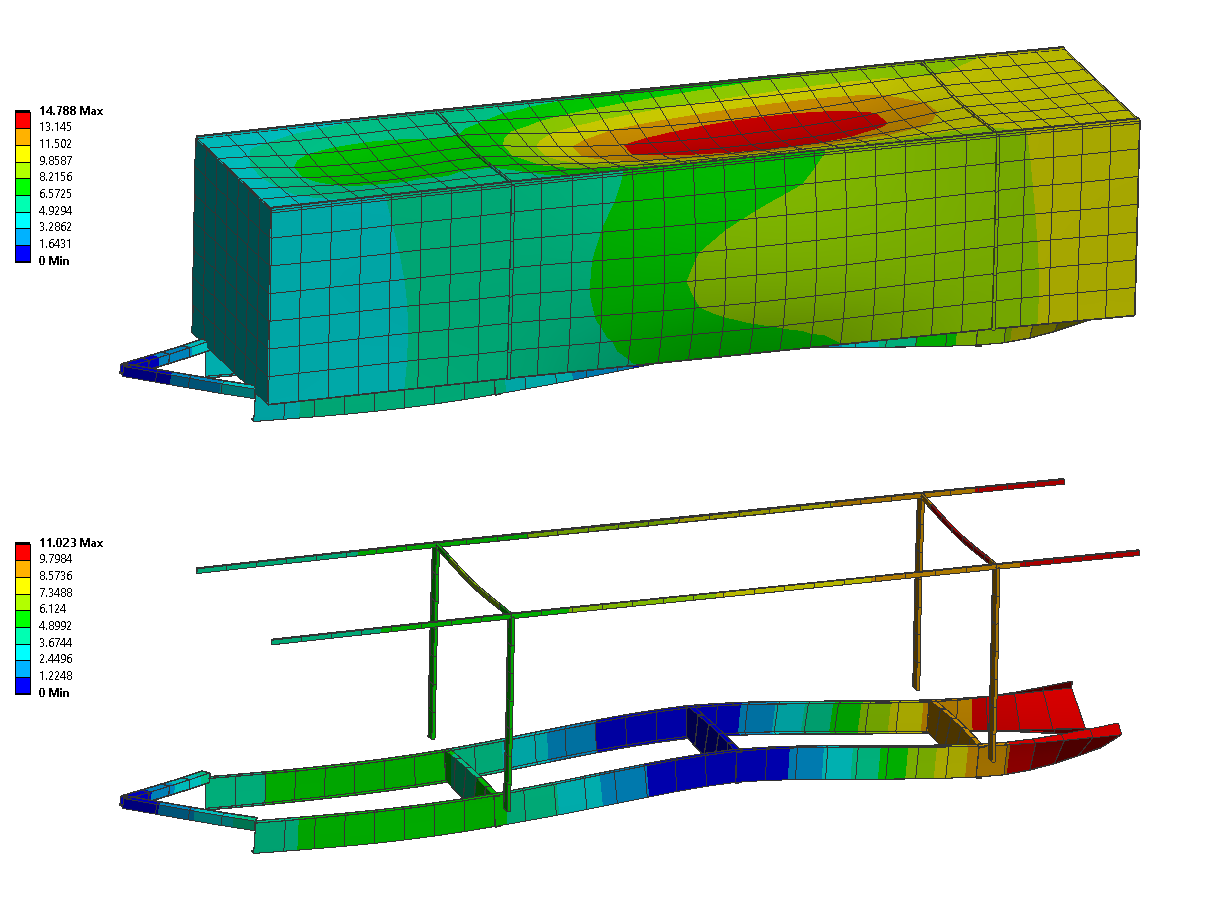
\includegraphics[width=1\linewidth]{04_figures/FEM 1.1.png}
  \caption{Deformation des Solar Butterflys im Lastfall der vertikalen Beschleunigung}
  \label{FEM 1.1}
\end{figure}

\subsubsection{Deformation - Lastfall 1.3 Longitudinale Beschleunigung}
\begin{figure}[H]
  \centering
  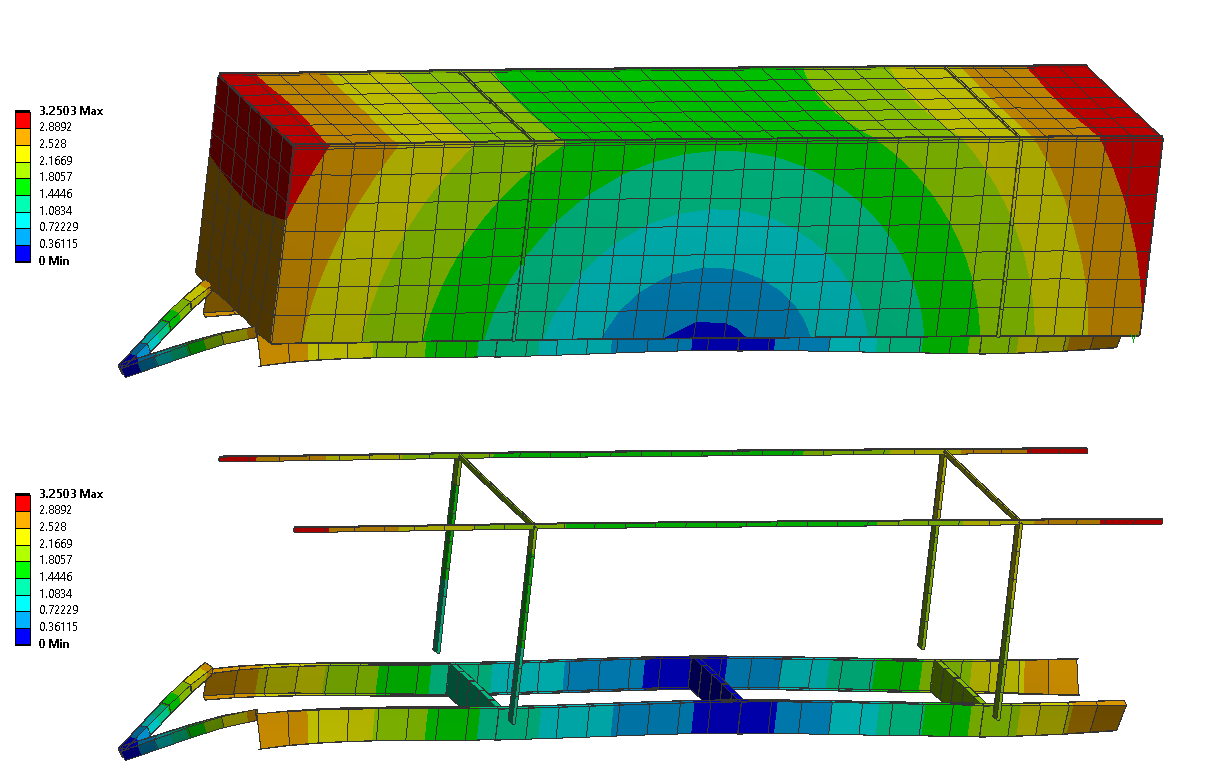
\includegraphics[width=1\linewidth]{04_figures/FEM 1.2.png}
  \caption{Deformation des Solar Butterflys im Lastfall der lateralen Beschleunigung}
  \label{FEM 1.3}
\end{figure}

\subsubsection{Deformation - Lastfall 1.4 Laterale Beschleunigung}
\begin{figure}[H]
  \centering
  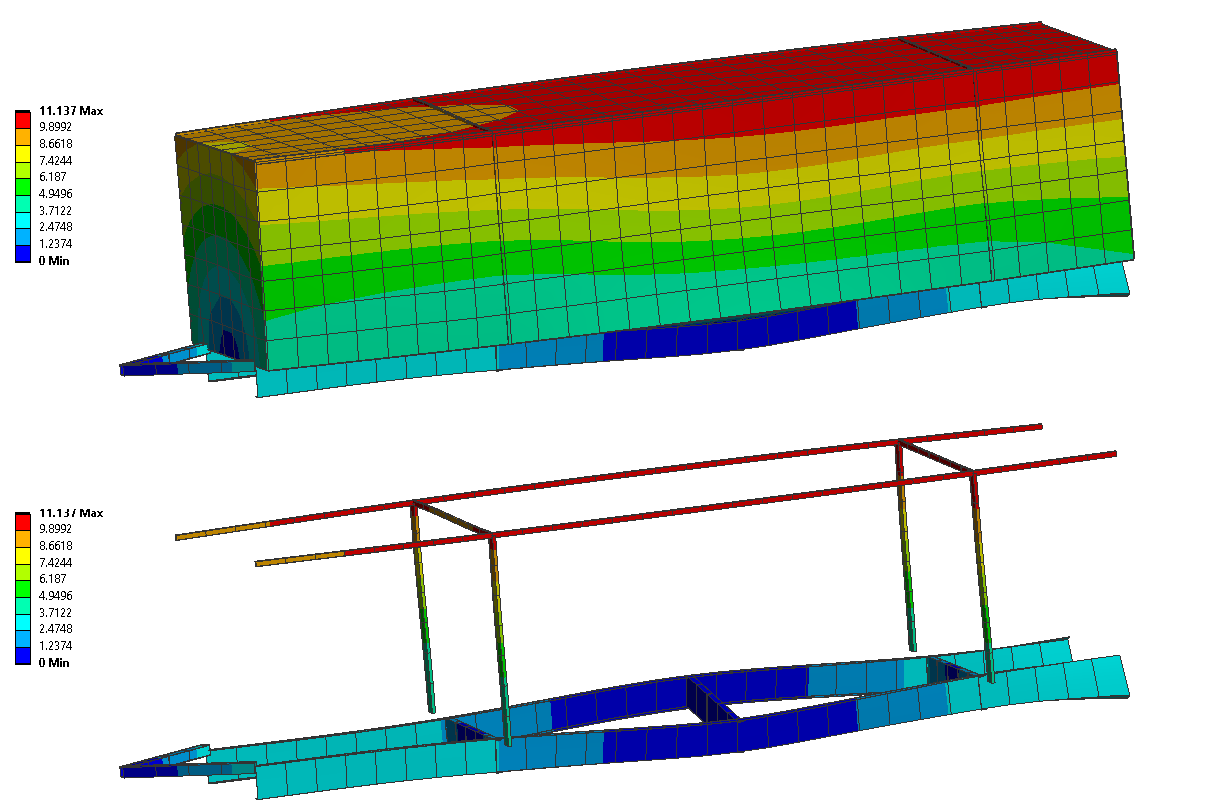
\includegraphics[width=1\linewidth]{04_figures/FEM 1.4.png}
  \caption{Deformation des Solar Butterflys im Lastfall der longitudinalen Beschleunigung}
  \label{FEM 1.4}
\end{figure}

\subsubsection{Deformation - Lastfall 1.5 Rotatorische Beschleunigung}
\begin{figure}[H]
  \centering
  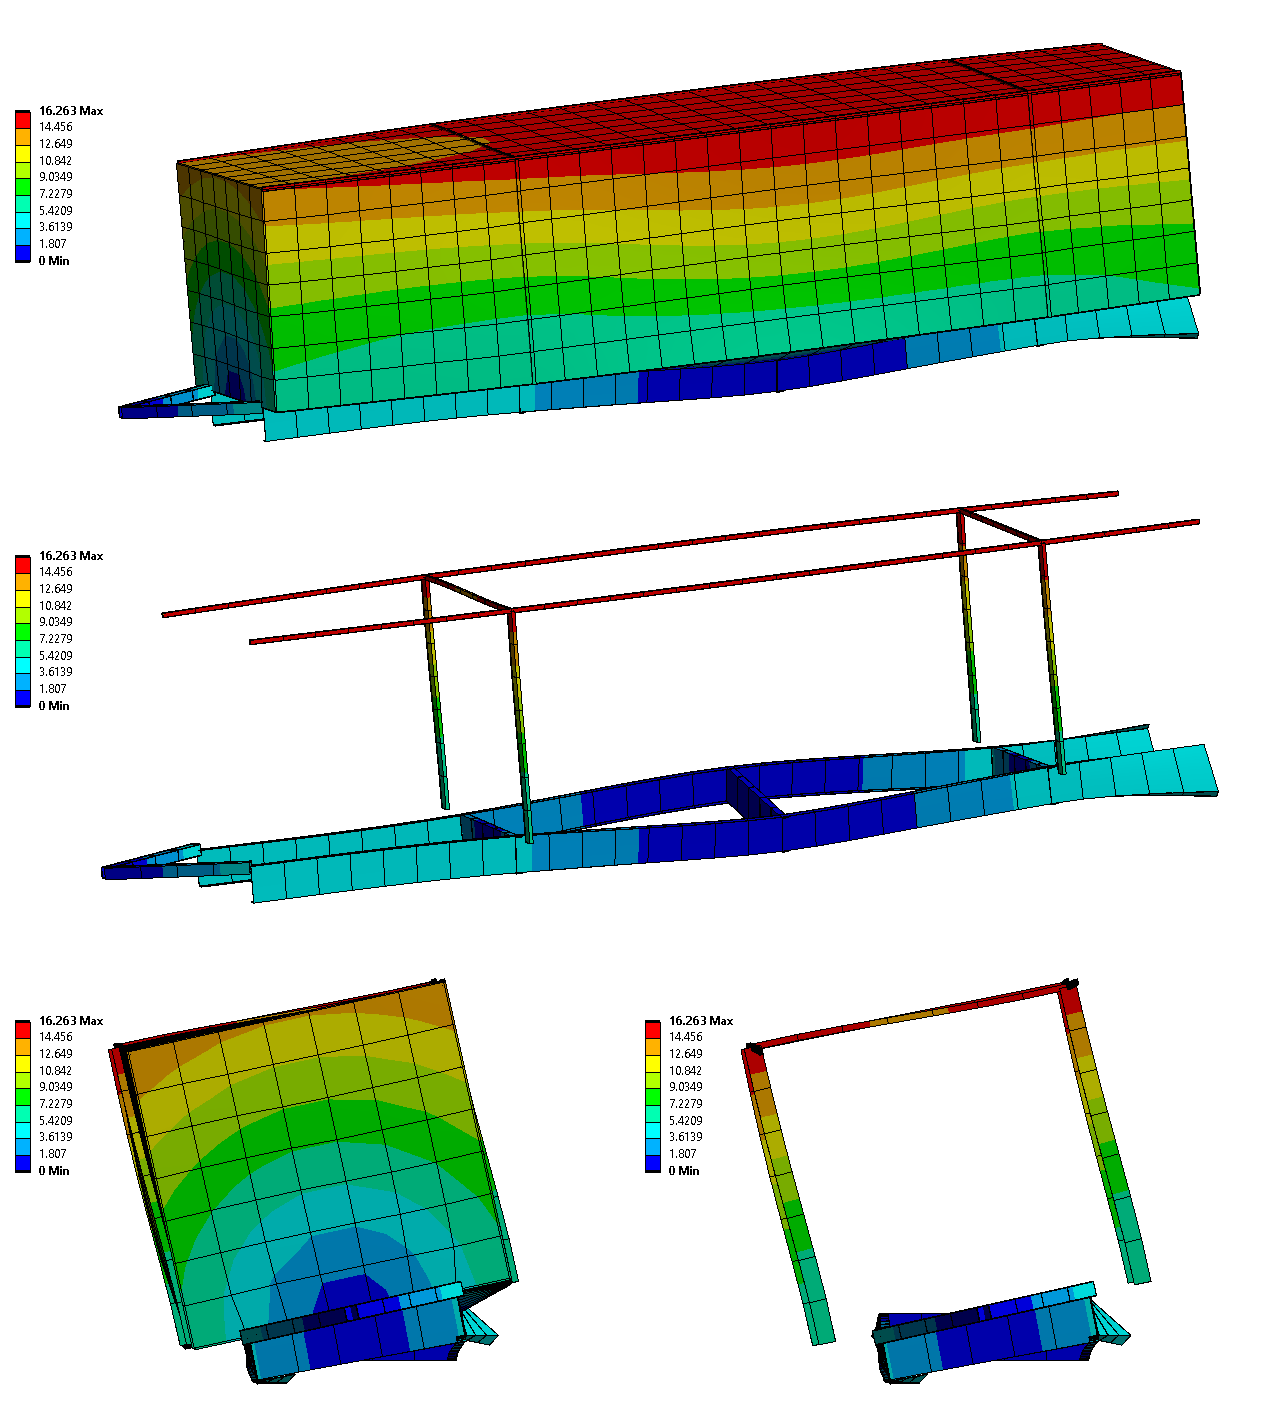
\includegraphics[width=1\linewidth]{04_figures/FEM 1.5.png}
  \caption{Deformation des Solar Butterflys im Lastfall der rotatorischen Beschleunigung}
  \label{FEM 1.5}
\end{figure}
\newpage


  \part{Elektronischer Anhang}
  \appendix
  \section{Bilder des Solar Butterflys}
\label{Bilder des Solar Butterflys}



\section{Dokumente aus fremden Arbeiten}
  \subsection{Anforderungsliste}
  \label{e:Anforderungsliste}
  \subsection{Gewichtsberechnung}
  \label{e:Gewichtsberechnung}




\section{Datenblätter}
  \subsection{Materialien}
  \label{e:Materialien}
    \subsubsection{TDS Airex-T92}
    \label{e:Airex}
    \subsubsection{TDS Sikafles 552-AT}
    \label{e:Sikaflex}

  \subsection{Komponenten}
    \subsubsection{Federkennlinie-Hysterese}
    \label{e:Federkonstante}



\section{Berechnungen}
\label{e:Berechnungen}
  \subsection{Lastenheft - Beschleunigungen}
  \label{e:Lastenheft}
  \subsection{Handrechnungen}
  \label{e:Handrechnungen}
  \subsection{Dimensionierung}
  \label{e:Dimensionierung}
  \subsection{Dimensionierung Solarpanelen}
  \label{e:Solarpanelen}



\section{FEM}
  \subsection{FEM-Modell - Solarpanelen}
  \label{e:Panelen}
  \subsection{FEM-Modell - Solar Butterfly Global}
  \label{e:Globales FEM}
  \subsection{FEM Auswertung}
  \label{e:FEM Auswertung}

\end{document}
